% LaTeX Template for CPSC-298 Research Paper 
% Based on ACM SIGCONF template

% Force hyperref to use colored links (before loading acmart)
\PassOptionsToPackage{colorlinks=true,linkcolor=black,citecolor=blue,urlcolor=blue}{hyperref}

% Use screen option to enable colored links in ACM template
\documentclass[sigconf,screen]{acmart}

% Remove ACM copyright/conference info for student papers
\settopmatter{printacmref=false}
\renewcommand\footnotetextcopyrightpermission[1]{}
\setcopyright{none}
\acmConference[CPSC-298 Wikipedia Governance]{Wikipedia Governance Research}{2025}{Chapman University}
\pagestyle{plain}

% Packages you might need
\usepackage{graphicx}
\usepackage{url}       % For \url{} inline links
\usepackage{hyperref}
\usepackage{booktabs}  % For nice tables

% Configure link colors for better visibility
% Use AtBeginDocument to override ACM template settings
\AtBeginDocument{
    \hypersetup{
        colorlinks=true,       % Color text instead of boxes
        allcolors=.,          % Use current text color as default
        linkcolor=black,       % Internal links (sections, figures) - keep black
        citecolor=blue!50!black,   % Citations - navy blue
        urlcolor=blue!50!black,    % URLs and \href links - navy blue
        filecolor=blue!50!black    % File links - navy blue
    }
}

% Title and author information
\title{Anonymity and Free Speech: How Political Context Shapes Wikipedia Editors}
\subtitle{CPSC-298 Wikipedia Governance Research Project}

\author{Dylan Boswell, Kal Fernande, Emma Kochenderfer}
\affiliation{%
  \institution{Chapman University}
  \city{Orange}
  \country{USA}
}
\email{your.email@university.edu}

% Abstract
\begin{abstract}
% Abstract: 150-250 words summarizing your entire paper
% Include: problem, methods, key findings, contribution

Wikipedia aims to be a public encyclopedia, a place where people can share knowledge for the greater good. While its intentions- and those of most contributors– are noble, a few bad actors can move such a resource from being a public square– one where the sharing of information is done respectfully for the pursuit of the truth– to a tool to spread propaganda, misinformation and defamation for their own personal gain. Due to this problem, Wikipedia has incorporated an identification system, to track edits and comments on their wikipedia pages by a user’s IP address. This allows Wikipedia to at times restrict IP address editing access, if it is determined that a user is repeatedly vandalising the encyclopedia. While this system has successfully reduced the amount of spam and misinformation on the platform, it does bring up a series of other questions regarding user privacy, ease of contribution and user trust and has exposed a number of propagandised edits. We will research the link between Wiki and a user’s IP address for its impact on users who want to be critical of their government. Additionally, we’ll investigate the process of becoming a Wikipedia Administrator, how easy the role is to abuse, and what information administrators are privy to. Depending on that information, we’ll further research the meaning of this for a Wikipedia user who lives in a more repressive regime, and their trust in the wikipedia platform to preserve their anonymity. In asking these questions, we will determine the cost benefit analysis of anonymity versus spam protection to have the best outcomes for productive, constructive debate and discussion. We will then map the countries Wikipedia contributors come from and their respective laws protecting free speech and understand whether more draconian free speech laws are correlated with a decrease in wikipedia contributions and the impact of the IP address requirements.


\end{abstract}

% Keywords (relevant to your research)
\keywords{Wikipedia, governance, [add your keywords here]}

\begin{document}

\maketitle

% Main sections - each in a separate file
\section{Introduction}
% Introduction
% Structure: Problem/Motivation -> Background -> Research Questions -> Contributions -> Paper Outline

The main concept that we will be investigating throughout this paper is speech. The way that speech is expressed and restricted is a significant factor into determining human behavior. It is equally important in understanding the health of public squares, whether they even exist, and who contributes to them. In this paper, we will first analyze and discuss this concept as a whole, and understand the correlation between free speech laws and the sharing of information. Once we have established this link, we will analyze whether or not a sense of surveillance has a chilling effect on the contribution of the uncensored sharing of information. At this point, we will look to Wikipedia for our data analysis, as it is the most commonly used example of a public square. Due to its decentralized, open nature, it is not linked to one government or entity that could take punitive measures for free speech. This model is also responsible for how truth is found on Wikipedia, with multiple potentially anonymous editors attempting to extract data from opinion, and come to an unbiased conclusion on different topics. This makes it useful for our analysis, as it is an online public square, one where contributions are documented. We will use Wikipedia as a microcosm for a public square, one with global users and try to understand how different freedom of speech laws affect contributions to these public squares. We do this by tracking where Wikipedia contributions are coming from via IP address, and breaking down contributions by country. We then take data from the V-Dem democracy index to quantify freedom of speech laws country by country. 

% Research questions
This paper investigates the following research questions:
\begin{enumerate}
    \item Does surveillance have a chilling effect on speech in public forums? Is this dependent on enforcement or just the feeling of being surveilled? How does this relate to Wikipedia as a case study?
    \item Do freedom of speech laws have a chilling effect on the number of anonymous Wikipedia contributions?
    \item How do governance and administrative controls impact trust and anonymity?
\end{enumerate}

% Contributions
The main contributions of this work are:
\begin{itemize}
    \item Providing quantitative evidence to link free speech laws and Wikipedia edits.
    \item Show how governance mechanisms can impact participation and trust.
    \item Provide insights into balancing privacy and protection against vandalism in online public squares.
\end{itemize}

% Paper outline
The rest of this paper is organized as follows. 
Section~\ref{sec:related} reviews related work on Wikipedia governance. 
Section~\ref{sec:methodology} describes our data and methods.
Section~\ref{sec:results} presents our findings.
Section~\ref{sec:discussion} discusses implications and limitations.
Section~\ref{sec:conclusion} concludes and suggests future work.



\section{Related Work}
% Related Work
% Organize by themes/categories, not paper-by-paper
% Show how your work builds on, differs from, or fills gaps in existing work

\label{sec:related}

% Introduction to related work
Wikipedia’s unique open editing model offers an opportunity to research its governance in relation to politics and free speech laws.

% Subsection 1: First category of related work
\subsection{Wikipedia Governance and Community Culture}

Reagle's seminal work on Wikipedia culture~\cite{reagle2010good} examines the collaborative practices and governance mechanisms that enable Wikipedia's success. 

% Subsection 2: Second category of related work
\subsection{Wikipedia Trust and Reputation}
de Laat studied how Wikipedia monitors edits in order to avoid vandalism, with both admins and autonomous bots~\cite{de2014open}. Their paper states that Wikipedia experiences roughly 9000 vandalism edits daily, which is 7\% of all edits. It elaborates on institutional trust, which in this context is how Wikipedia approaches trusting contributors. Wikipedia uses backgrounding trust, which requires monitoring reputation and uses corrective mechanisms in the background to enforce norms, with sanctions placed on users who deviate. Bots are used to highlight edits that are potentially vandalism, which raises the question of bias within the automated bots. 

A paper on chilling effects showed that awareness of surveillance of IP address impacted Wikipedia usage, which is relevant because it means that potential editors/admins in more repressive countries will not participate to the full extent due to worries of surveillance~\cite{penney2016chilling}. The paper uses empirical backing to show the cost of spam control, with limits on edits, potentially especially for politically controversial pages.

\subsection{Wikipedia and Political Context}
The study done by Parra~\cite{parra2024righting} uses a casual inference framework and showed that politicians who switched from left to right wing parties had a drop in sentiment on their Wikipedia articles, which could show systematic political bias. This means that even with Wikipedia's monitoring of vandalism there is bias, making it important for us to study the role of free speech and politics with Wikipedia users. An Oxford paper found that the majority of articles about places were edited by people living in the UK, USA, France, Germany, and Italy~\cite{Oxford2015WikipediaWorldView}. Digital connectivity is a contributing factor, along with high income levels.

% Positioning your work
\subsection{Our Work in Context}

The majority of prior existing similar research examines survey-based measures; we are using quantitative empirical behavioral data to examine user participation on Wikipedia. Our research is primarily focused on observable edits and behavior. Additionally, we focus on several different countries and create a bridge between quantitative edit evidence and free speech laws related to those countries. This contributes to further understanding how free speech laws can impact user behavior in digital public squares like Wikipedia.


\section{Methodology}
% Methodology
% Be specific enough that someone could reproduce your work

\label{sec:methodology}

% Overview
Using the Wikipedia API, we will track edits from frequently visited versions of Wikipedia for different countries for edits made by unregistered users. We will use the IP addresses of those unregistered users to link them to that editor’s country. This will be used to compare edit frequency per country against benchmarks for free speech laws. Our benchmarks for free speech laws will be sourced from the V-Dem democracy index.

\subsection{Data Collection}

We used the Wikipedia API for frequently visited versions of Wikipedia for different countries. The versions that we are focusing on are Wikipedia en (English), es (Spanish), ru (Russian), and hu (Hungarian). These versions of Wikipedia were selected based upon availability of unregistered user edits.

% Example of how to cite a dataset or tool:
% We collected data from the Wikipedia API \cite{wikipedia-api} covering...

\subsection{Data Processing}

We filtered out edits made by registered users, as we do not have access to their IP addresses. Unregistered user edits were linked to their respective country by IP address, as seen in Figure~\ref{fig:totaledits}. Our data processing pipeline is available in our GitHub repository.\footnote{\url{https://github.com/kochenderferc/wikipedia-political-context}} We then accounted for population size using the Rest Countries API.\footnote{\url{https://restcountries.com/}}

\begin{figure}
    \centering
    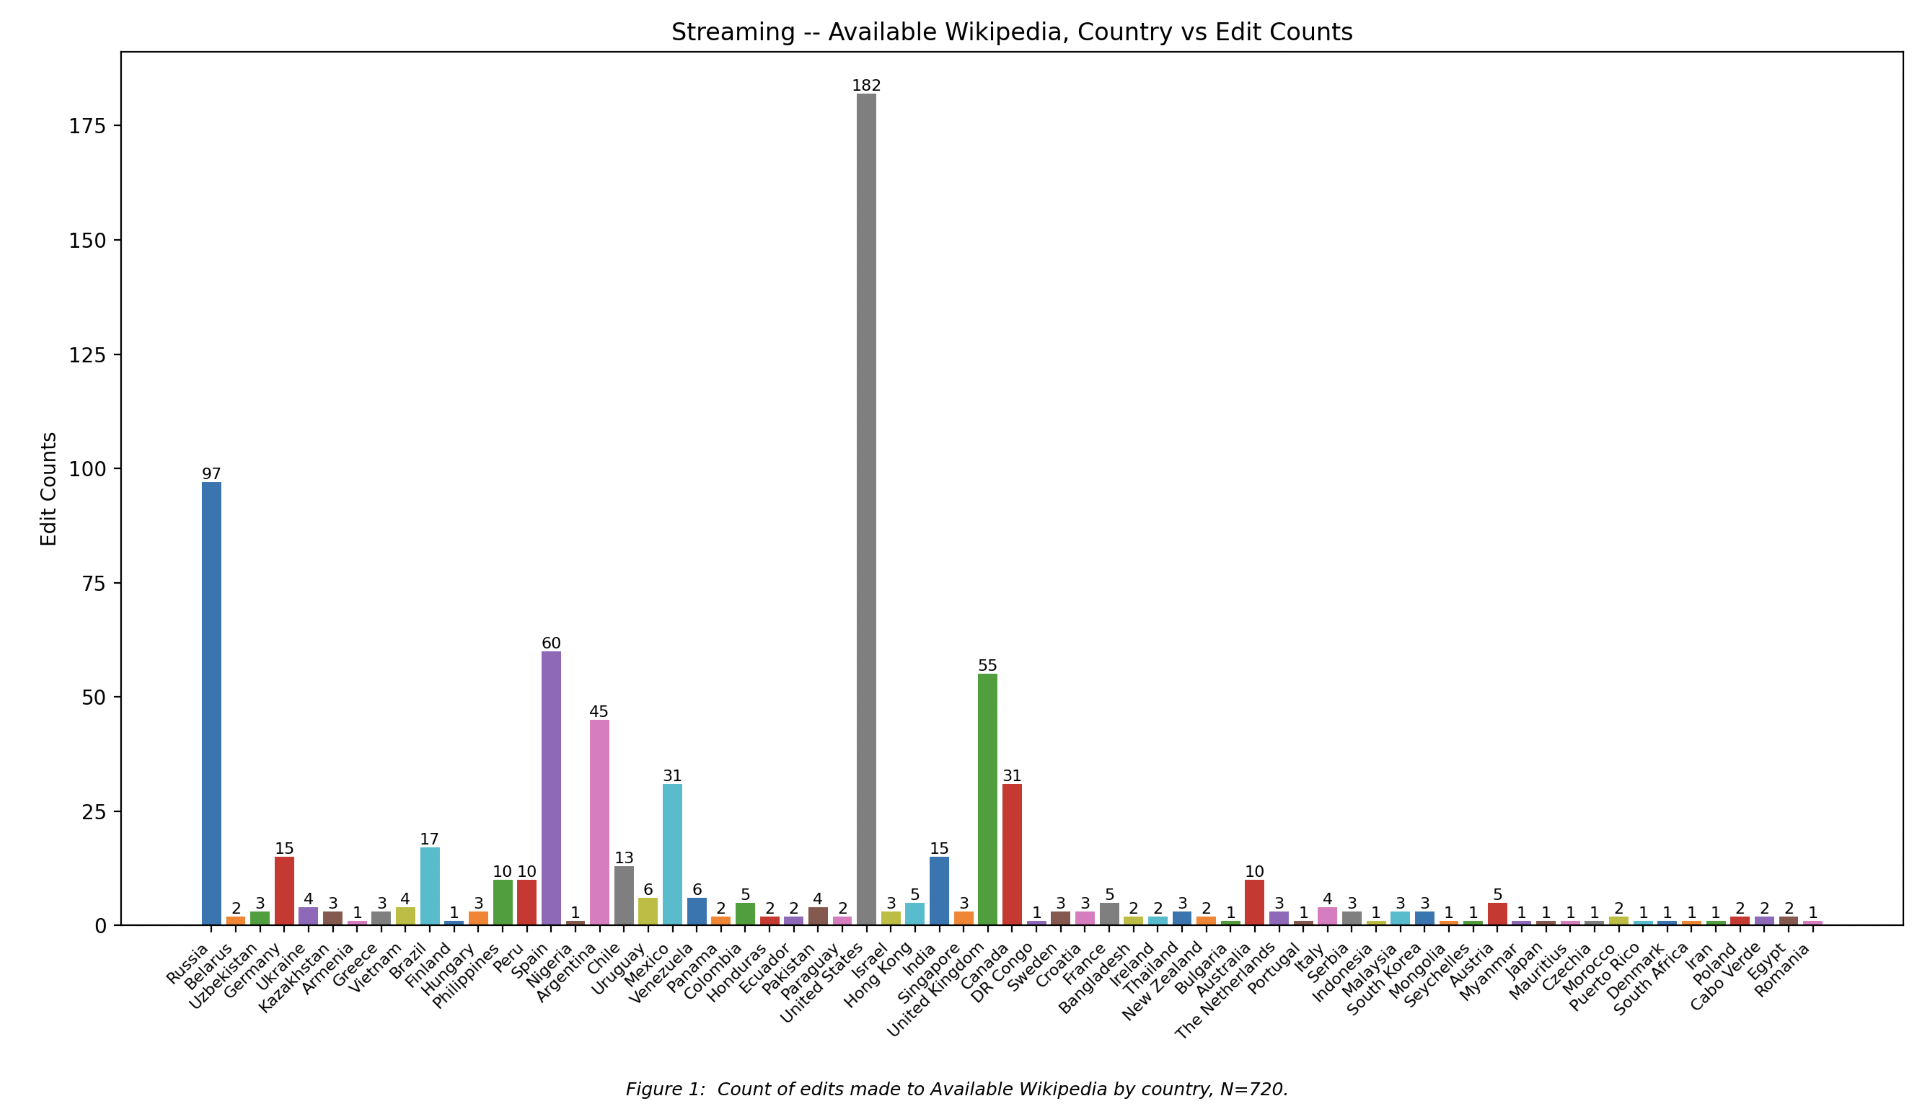
\includegraphics[width=\linewidth]{figures/totaledits.png}
    \caption{Unregistered Wikipedia edits per country}
    \label{fig:totaledits}
\end{figure}

\subsection{Analysis Methods}

We compared the results to the V-Dem (Varieties of Democracy) index to understand the link between freedom of speech and edits on Wikipedia. The relationship between liberal democracy and freedom of expression for 2023 is shown in Figure~\ref{fig:vdem}. This data for the selected Wikipedia countries was then overlaid with our data on unregistered edits, after accounting for population size. Our comparison prior to accounting for population size is shown in Figure~\ref{fig:initialcomparison}.

\begin{figure}
  \centering
  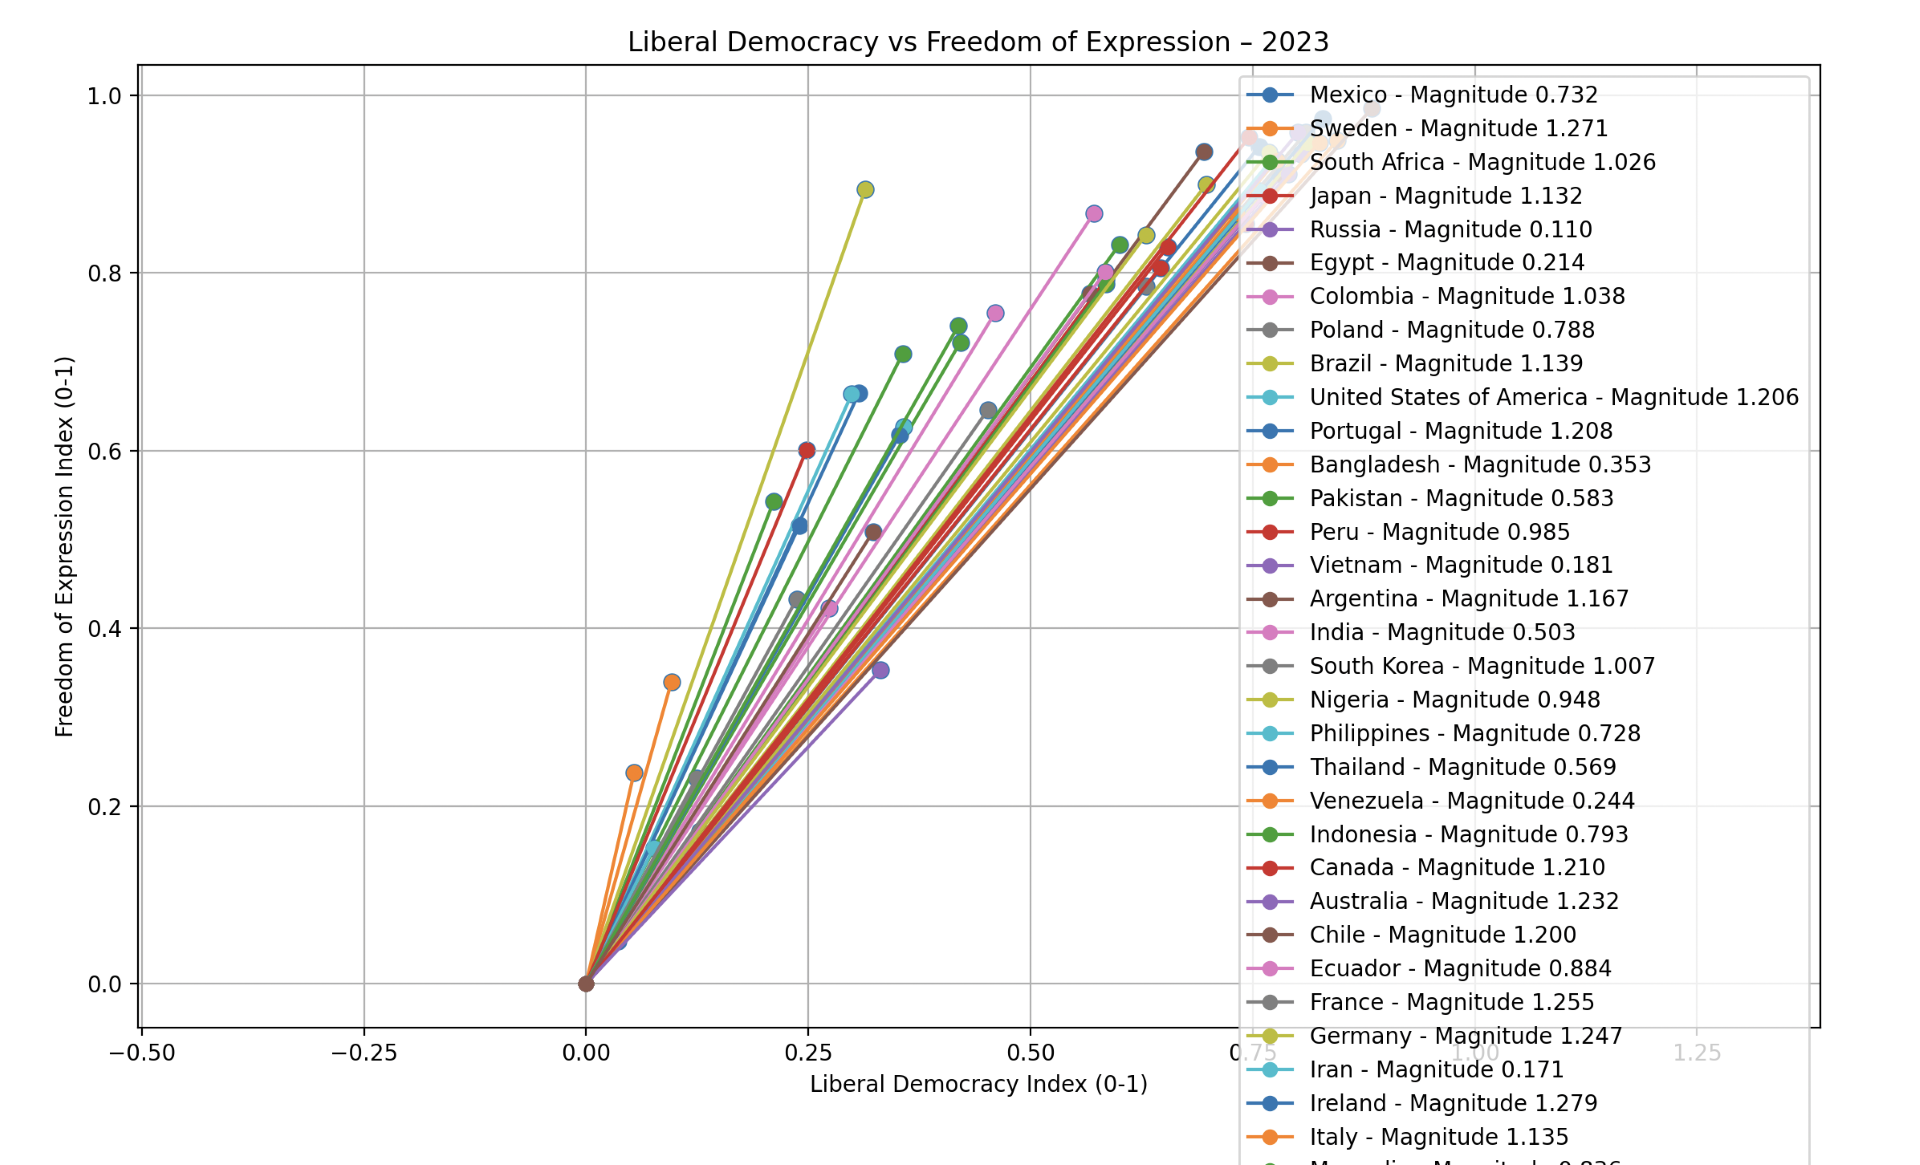
\includegraphics[width=\linewidth]{figures/vdem.png}
  \caption{Liberal Democracy vs. Freedom of Expression from the V-Dem index for 2023}
  \label{fig:vdem}
\end{figure}

\begin{figure}
    \centering
    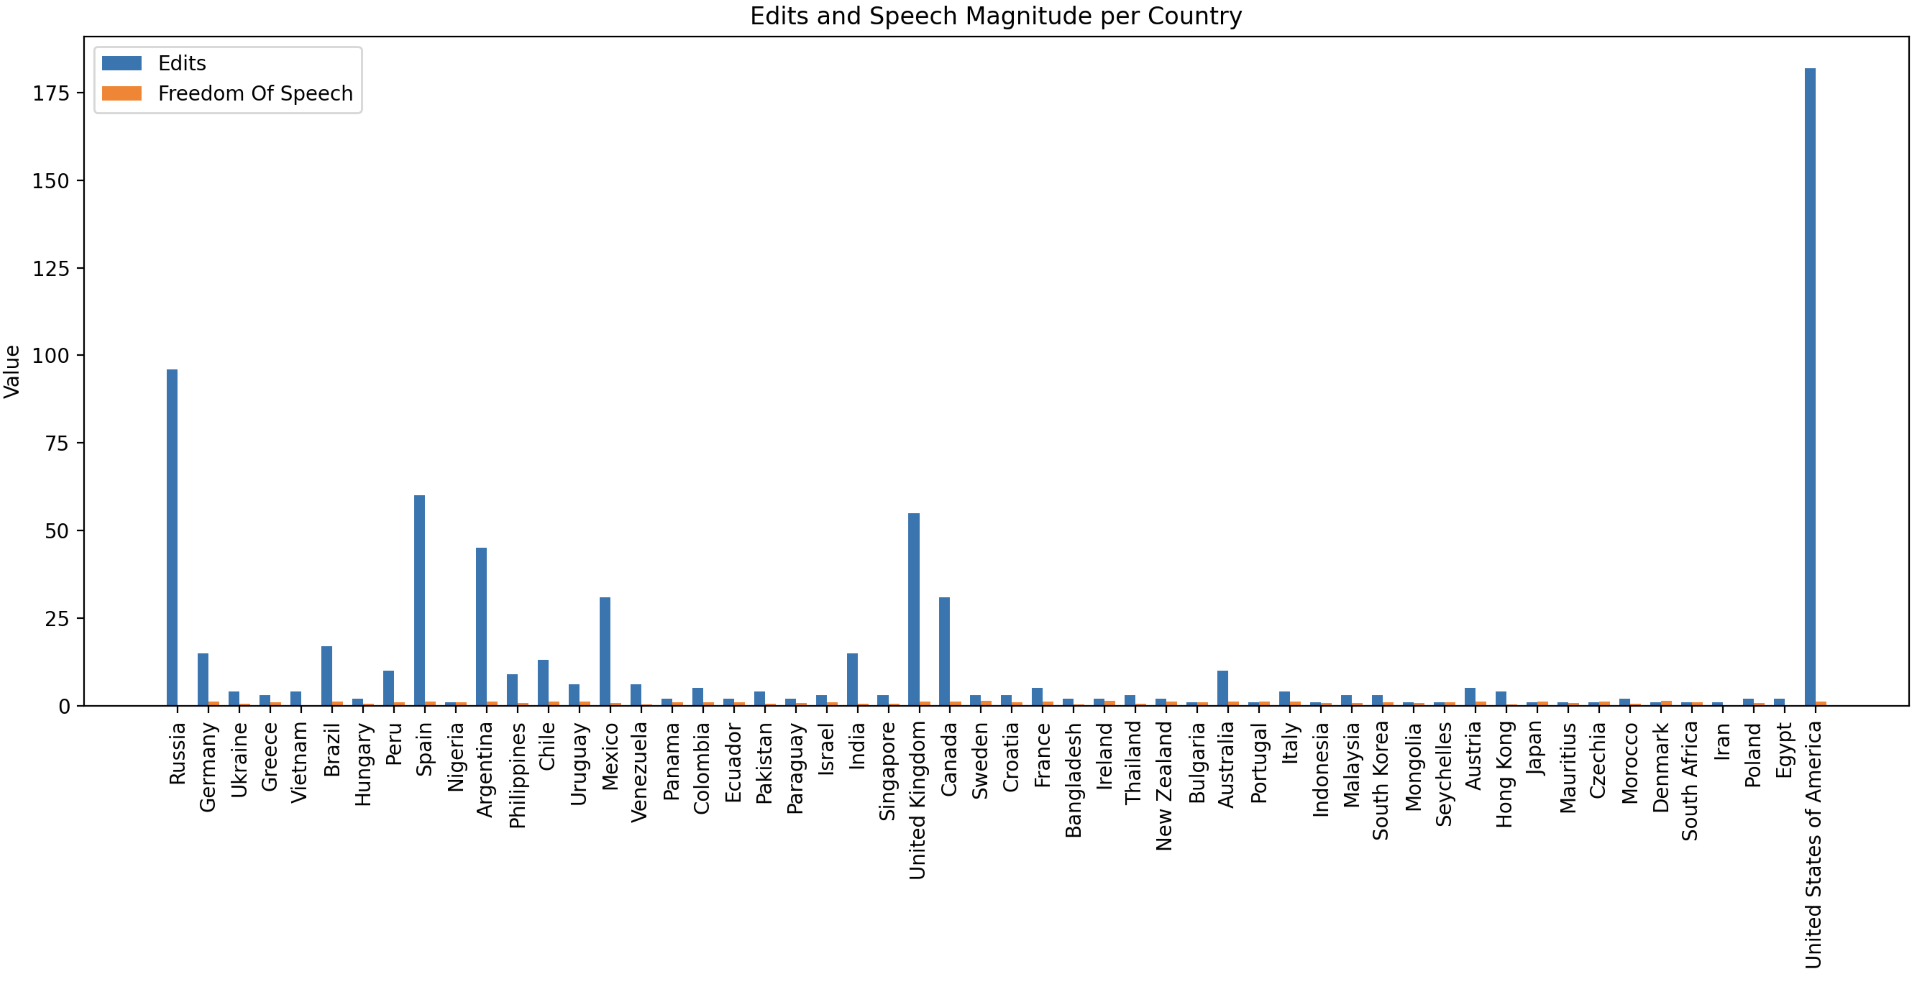
\includegraphics[width=\linewidth]{figures/initialcomparison.png}
    \caption{Initial comparison between unregistered edits and freedom of speech}
    \label{fig:initialcomparison}
\end{figure}

% If you have equations, you can include them:
% \begin{equation}
% your\_formula = here
% \end{equation}

\subsection{Ethical Considerations}
All data consists of publicly available Wikipedia content accessed in compliance with \href{https://foundation.wikimedia.org/wiki/Policy:Terms_of_Use}{Wikimedia's Terms of Use}.



\section{Results}
\input{sections/results}

\section{Discussion}
\input{sections/discussion}

\section{Conclusion}
\input{sections/conclusion}

% Acknowledgments (optional)
\section*{Acknowledgments}
We thank \dots for \ldots.

% Bibliography
\bibliographystyle{ACM-Reference-Format}
\bibliography{references}

% Appendix for AI Usage Documentation
\appendix
\section{AI Usage Documentation}
\input{sections/appendix-AI-usage}

\end{document}

